\subsection{The interdependence assumption}\label{subsec:interdependence}

Let $\bar{\mathcal{M}}$ be a joint distribution from which the random variables
$(s, r)$ are drawn. We say that $s$ and $r$ are interdependent when there exist
$s_1, r_1$ and $s_2, r_2$ in the support of $\bar{\mathcal{M}}$ with $s_1 \neq
s_2$ such that:

\begin{align*}
    \Pr[(s, r) = (s_1, r_1)] &< \Pr[(s, r) = (s_1, r_2)]
\land\\
    \Pr[(s, r) = (s_2, r_1)] &> \Pr[(s, r) = (s_2, r_2)]
\end{align*}

Where the pair $(s, r)$ is drawn from the joint distribution
$\bar{\mathcal{M}}$.

It is clear that when two random variables $s$ and $r$ exhibit interdependence,
they must necessarily be dependent random variables. To see that
interdependence is a stronger version of dependence, observe that in the case
of dependence, the probability for some $s = s_1$ conditioned on $r = r_1$ is
necessarily different from the probability for some $s = s_2$ conditioned on $r
= r_2$. In interdependence, it can be seen that we additionally require the
event $s = s_1$ which was less probable than the event $s = s_2$ under the
condition $r = r_1$ to become more probable than $s = s_2$ under the condition
$r = r_2$.

We observe that commonly compressed texts such as HTML content exhibit
interdependence almost everywhere. To be more precise, if we sample, for
example, digrams (two-letter sequences) in HTML content of popular websites and
treat this two-letter sequence $\phi = (s, r)$ of the two characters $s$ and
$r$ as a random variable $\phi$, we notice that $s$ and $r$ are dependent
variables and in fact interdependent. Similarly when sampling two-word sequences
$\phi = (s, r)$ of the two words $s$ and $r$ from English literature, then $s$
and $r$ are interdependent. The same occurs for digrams in English. This
straightforward fact is supported by extensive statistical analyses in the
scientific literature such as \cite{mayzner1965tables}.

While the interdependence assumption is a general notion observed in all common
plaintexts, it is suitable to mention here how these ideas will emerge as we
mount our attack. In a plaintext $(s, r)$ in which the attacker controls some
reflection string $r$ and wishes to obtain information about some secret string
$s$, she wishes to distinguish between the cases $s = s_1$ and $s = s_2$ of two
different secrets $s_1$ and $s_2$, i.e. between the instances $(s_1, r)$ and
$(s_2, r)$. By measuring the difference in the probability of $(s, r)$
occurring for $r = r_1$ and $r = r_2$, the attacker can distinguish which value
of $s$ is in use. If $s = s_1$, then the attacker will observe the inequality
$\Pr[(s, r) = (s_1, r_1)] < \Pr[(s, r) = (s_1, r_2)]$, but when $s = s_2$, the
attacker will observe the different inequality $\Pr[(s, r) = (s_2, r_1)] >
\Pr[(s, r) = (s_2, r_2)]$.

The necessity of the assumption that the plaintext being compressed follows an
interdependent distribution will become clear shortly, when we introduce our
definition of compression functions. This will also immediately hint at how the
attacker is able to perform these measurements of probability inequalities
indirectly by observing ciphertext lengths.

\subsection{Composing with compression}\label{subsec:comcompose}

We now shift our interest to algorithms which compose compression and
encryption. We define the composition of a compression algorithm with a
rendering function and an encryption algorithm.

The encryption scheme above is treated as a composition of a
compression and encryption algorithm:
\begin{equation*}
    \mathcal{E} = \textrm{Enc} \circ \textrm{Com}
\end{equation*}

$\textrm{Com}$ is any polynomially computable reversible function that takes an
input string and outputs a new string: $\textrm{Com}: \{0, 1\}^* \leftarrow \{0,
1\}^*$.

$\textrm{Enc}$ denotes an encryption function. We stress our important
assumption that $\textrm{Enc}$ is defined on $\{0, 1\}^*$ and not on some
fixed-length input.

The composition of the compression function $\textrm{Com}$ and the rendering function $f$
is defined:
\begin{equation*}
    \mathcal{K} = \textrm{Com} \circ f
\end{equation*}

We call $\mathcal{K}$ an editing function. For the rest of the paper, we treat
$\mathcal{K}$ as a compression function.

\subsection{Compression idealness}\label{subsec:com_idealness}

We now move on to define the notion of compression idealness.

Let $\mathcal{K}$ be a function defined on some domain and with output space
all strings $\{0, 1\}^*$, and let $\bar{\mathcal{M}}$ be a distribution whose
support is a subset of the domain of $\mathcal{K}$.  We say that $\mathcal{K}$
is an ideal compression function with respect to the distribution
$\bar{\mathcal{M}}$ when for every $w_1, w_2$ in the support of
$\bar{\mathcal{M}}$ we have:

\begin{equation*}
\Pr[w = w_1] < \Pr[w = w_2] \iff \lvert\mathcal{K}(w_1)\rvert > \lvert\mathcal{K}(w_2)\rvert
\end{equation*}

Where $w$ is a random variable drawn from $\bar{\mathcal{M}}$.

The intuitive notion behind compression idealness is that the encoding
function is somehow perfectly aware of the input distribution. It
exploits this knowledge of the input space to encode each possible
input in an ideal way – more often occurring plaintexts are compressed
better, i.e. in shorter length, than rarely occurring plaintexts.
Practical compression functions are not perfectly ideal, because the
distribution of plaintexts they try to cover is broad and ill-defined.
However, such compression functions try to learn the distribution of
the plaintext they are about to compress by observing frequencies of
occurrences and taking advantage of them.

We now turn our attention to two specific compression functions, the
LZ77 and Huffman function. These two compression functions are of
interest for two reasons. First, they are representative of the way
typical lossless compression functions work internally, by taking
advantage of letter frequencies (Huffman) or letter-sequence
repetitions (LZ77). Second, they are the ones almost exclusively used in
practice. The DEFLATE algorithm \cite{deutsch1996deflate}, which is a composition of LZ77 and
Huffman, is the algorithm used in gzip, which is prevalent on the
modern web. In 2016, 98.85\% of websites that enabled compression used
some form of gzip. We argue that both LZ77 and Huffman are nearly
ideal compression functions. The complexity of the Huffman and
especially the LZ77 algorithms arises from many intricate technical
details, such as, for instance, the sliding window size of LZ77. These
details make it impractical to deal with these functions in analytical
proofs.

We support our idealness claims in an experimental manner. Our experiment
measured the compression performance of the Huffman and an ideal function on a
text of English literature\footnote{The screenplay of the movie "The Social
Network".}. First, we calculated the occurences of each character (letters and
digits) in the text. Second, we generated the Huffman
table for this text and the table of an ideal function based on the character
frequencies. Each character is represented by a bitstream in both tables. Figure
\ref{fig:huffman_idealness} depicts the length of the bitstreams of characters
in descending order of occurencies for both the ideal and the Huffman functions.

    \begin{figure}[thpb]
        \centering
            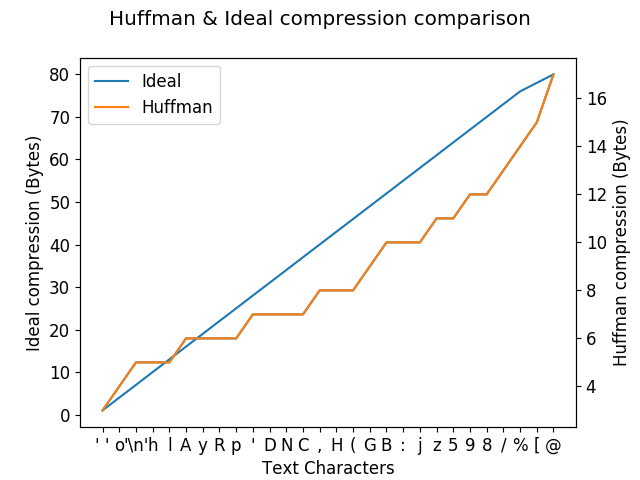
\includegraphics[width=0.48\textwidth]{idealness_experiments/huffman_idealness.png}
        \caption{Comparison between Huffman and ideal compression}
        \label{fig:huffman_idealness}
    \end{figure}

\subsection{Length monotonicity}\label{subsec:lenmonotone}

An important assumption for our attack is that the encryption function
$\textrm{Enc}$ is \textit{length monotonic}. Specifically, for any keys $k_1
k_2$ in the key generating function space and string messages $m_1, m_2$:

\begin{equation*}
\begin{split}
|m_2| > |m_1|
\Rightarrow
|\textrm{Enc}_{k_1}(m_2)| \geq |\textrm{Enc}_{k_2}(m_1)|
\end{split}
\end{equation*}

If the last inequality becomes strict, we call the encryption function
\textit{strictly length monotonic}.

A practical instance of a length monotonic encryption function is AES \cite{standard2001announcing}.
Stream ciphers can be treated as strictly monotonic to the bit level.

\subsection{Compressibility with respect to predicates}\label{subsec:propertycom}
In this section we will define compressibility with respect to predicates. We
show that all ideal compression functions that exhibit interdependence are
compression detectable by a reflection vector $\overbar{r}$ with respect to a
predicate $Q$ and a distribution $\mathcal{M}$

Let $\mathcal{M}$ be a plaintext distribution and $Q(s)$ be a predicate on the
plaintext $s$ drawn from $\mathcal{M}$. Furthermore, we require that $Q$ is not a
trivial predicate; that is, there must exist elements for which $Q$ is true and
others for which it is false.  Let us use $\mathcal{M}_Q$ to denote the
distribution $\mathcal{M}$ conditioned on the predicate $Q$.

For the specific property $Q$ and plaintext distribution $\mathcal{M}$, define:
\begin{equation*}
    \pi \defeq max(\Pr[Q(s)], 1 - \Pr[Q(s)])
\end{equation*}

Where $s$ is drawn from $\mathcal{M}$.

Let $\overbar{r} = (r_1, r_2) \in \mathcal{M}^2$ be a reflection string pair,
$\mathcal{K}$ be an ideal compression function, $f$ be a rendering function, and
let $\alpha(\lambda)$ be a non-negligible function.

We now examine how the lengths of compressing a secret $s$ rendered with
reflection strings $r_1$ and $r_2$ respectively compare.

The predicate $Q$ partitions the set $\mathcal{M}$ into two partitions
$\mathcal{M}_Q$ and $\mathcal{M}_{\lnot Q}$. We are interested in reflection
string pairs $\overbar{r} = (r_1, r_2)$ for which the comparison direction
depends on which partition $s$ belongs to.  If $s \in \mathcal{M}_Q$, it should
compress better when reflection $r_1$ is used as compared to when $r_2$ is used.
On the contrary, if $s \in \mathcal{M}_{\lnot Q}$, the opposite direction should
occur.  If this is the case for the selected reflection pair, we say that $Q$
compares favourably under $\overbar{r}$:

\begin{equation*}
\begin{split}
    cpr^Q_{\mathcal{K}}(s, \overbar{r})
    \defeq\\
    \begin{cases}
        |\mathcal{K}(s, r_1)| < |\mathcal{K}(s, r_2)| &\text{ if } Q(s)\\
        |\mathcal{K}(s, r_1)| \geq |\mathcal{K}(s, r_2)| &\text{ otherwise}
    \end{cases}
\end{split}
\end{equation*}

The reflection pair $\overbar{r}$ \textit{detects} predicate $Q$ under
compression function $\mathcal{K}$ over the secret distribution $\mathcal{M}$ with
advantage $\alpha$ when the comparison is favourable for both $s_1$ drawn from
$\mathcal{M}_Q$ and $s_2$ drawn from $\mathcal{M}_{\lnot Q}$. Formally, we
define the predicate $dtc_\alpha(Q, \overbar{r}, f, \textrm{Com}, \mathcal{M})$
as follows:

\begin{align*}
    \Pr
        [cpr^Q_{\mathcal{K}}(s_1, \overbar{r}) \land
         cpr^Q_{\mathcal{K}}(s_2, \overbar{r})]
    \geq\\
    \pi + \alpha(\lambda)
\end{align*}

Where $s_1$ is drawn from $\mathcal{M}_Q$ and $s_2$ is drawn from
$\mathcal{M}_{\lnot Q}$.

We call $Q$ \textit{compression-detectable} with an advantage $\alpha$ if a pair
$\overbar{r} = (r_1, r_2)$ exists, such that $dtc_\alpha(Q, \overbar{r}, \mathcal{K},
\mathcal{M})$ holds. Furthermore we require that such a pair $\overbar{r}$ is
polynomially computable. That is, there exists some polynomial-time
functionality $\mathcal{O}_R(\mathcal{K}, Q, \mathcal{M})$ which produces an
$\overbar{r}$ such that $dtc_\alpha(Q, \overbar{r}, \mathcal{K}, \mathcal{M})$ holds.

The compression-detectability property exists in all common compression
functions as long as $s$ and $r$ compress in the same context. We will now
prove the fact that all compression functions which are ideal under some
distribution $\bar{\mathcal{M}}$ exhibit compression-detectability of some
predicate $Q$.

\subsection{Good compression allows predicate detection}

We now move on to show that all good compression functions exhibit
compression-detectability of some predicate. In intuitive terms, this means
that if a compression function compresses well enough, it will necessarilly
allow one part of the plaintext to affect how another part of the plaintext
compresses. An attacker that is able to measure how well a string compresses
can use this to detect a predicate on the second part of the plaintext by
changing the first part of the plaintext.

More specifically, we model our plaintext input to the compression function as
the usual pair $(s, r)$ consisting of the secret string $s$ and reflection
string $r$. When $(s, r)$ are encoded by a compression function $\mathcal{K}$ ideal
under some plaintext distribution $\bar{\mathcal{M}}$, a simple predicate
allows the distinction between two secrets $s_1$ and $s_2$ using a reflection
pair $(r_1, r_2)$.

In the following theorem, we prove compression detectability of a predicate
with the following simplifications. We make the assumption that the
resulting reflection pair $(r_1, r_2)$ is computable.

\begin{lemma}[Good compression is detectable]
Let $\mathcal{K}$ be an ideal compression function with respect to some
interdependent distribution $\bar{\mathcal{M}}$. Then there exists
some compression-detectable predicate $Q$ for $\mathcal{K}$.
\end{lemma}

A full proof can be found on Appendix A.
